\color{blue}

\section{人机交互}
(备注:作为“人机强交互”的印子,可以简略介绍)

人机交互研究最初是以机器为中心, 心理学家训练选拔员工以适应机器。后来二战期间机器复杂到难以使人适应, 研究重心才转移到以人为中心……[\cite{} 人机交互研究综述,2017]

人机交互有多种形式, 从最初的发展到现在经历了三代的更替,更替的过程彰显了从“硬交互”到“软交互”的过程。 第一个交互时代是鼠标加键盘的时代……第二个交互时代是触摸交互时代, 使人们的双手从键盘和鼠标中解放出来, 人与机器的交互变得更 加 直 接 和 简 单 ……第三个交互时代是感官交互时代,在这个时代,人机交互已经不需要直接的接触,身体控制、感官交互占据主流……[\cite{}, 新媒体语境下的人机交互叙事初探,2018]。人类与机器间的共生合成体可以说是正在形成……而这种合成体威胁了我们这种感觉的稳定性。 人类创造了电脑,接着电脑又创造了新型的人,这也许正在悄然发生。[\cite{}马克·波斯特.信息方式[M].范静哗.译,北京:商务印书馆,2000:11 ]


======

(可参考 Possible Effects of Internet Use on Cognitive Development in Adolescence\cite{Mills2016})
\section*{信息爆炸会导致认知障碍}
信息本身爆炸式的增长了,随着互联网,特别是移动互联网的发展,人们产生
信息和内容的方式发生了巨大的变化。该点又可以从如下三个方面进行说明。

a)比如原来的论坛或者博客,乃至门户网站,其信息都是定时更新。而有了微博,微信则变成了随时,随地的都可以发送信息和图片等。即信息发送本身不再受空间,时间的限制了;

b)再次,由于有了关注和交互,任何一个内容的产生我们可以有大量的转发和评论,而评论本身即是对信息内容的再次加工,又变成了一条信息的信息,大V或网红发送信息或热点事件本身,往往会产生大量指数级增长的评论信息,这本身也是信息爆炸的一个点;

c)另外还有就是随着物联网和传感技术的发展,我们采集信息或数据的方式发生了巨大的变化,比如对于温度,水压检测,我们可以通过传感器实时的采集数据,而不是类似传统方式定时人工记录,这些自动化采集技术的发展本身也极大增加了信息扩张的速度


第二个是基于被动推送的信息获取方式

即我们常说的微博,微信,知乎等平台,而这些平台基本都是通过关注他人或关注话题获取到实时的信息推送,这些信息推送往往是一种被动的信息接收过程。或者说这些渠道占据了我们一天绝大部分的信息来源,导致我们连类似新浪的门户新闻网站往往都懒得再看。

我们能接收到的信息往往受到我关注的人,特别是大V的影响,如果这些人没有产生或推送出某条信息,那么在我们的TimeLine上往往就没有任何信息显示。虽然当前也有话题关注的功能,但是这个功能往往用的并不多,除非出现特别热门的话题,我可能才会进入到微博的话题关注中。

正是由于是对人的关注,而不是对知识点或内容本身的关注,我们发现很多高质量的内容往往并不会推送到你的时间线上,而如果有大V愿意转发你的内容,往往就容易引起一个指数级的引爆传播。同时由于我们是对人的关注,导致我们不得不被动接收该人发出的所有信息,比如我关注了一个IT专家,但是他可能每天更多发布的是儿子照片或美食图片,而不是我真正关心的内容,这本身也可能增加信息噪音。

由于我们是对人的关注,我们一方面更多获取的是大V加工后和处理后的信息,而不是最原始核心的知识结构,另外一方面就是我们由于常时间被动接受信息,思维更加容易受到他人影响而丧失独立思考。这些都是导致我出现认知瓶颈和障碍的核心原因。


\section{“强”交互}

机器和设备对于“人的影响”日益明显,甚至正在 “创造新型的人”,这和其本身的存在形式的演变不无关系。在现有的“人机交互”的基础上,我们尝试提出“强交互”的概念,并进一步探究“设备”对人的影响。
2.1、刺激强度
	设备对人刺激强度的不断增加是重要特点。
2.2、软件的“沉浸式设计”
	各类产品的“沉浸式设计”是加强人机交互强度的直接因素,这是一个涉及到心理、设计、游戏等领域的概念。
2.3、相互反馈
人机“强交互”语境下,存在一个人与机器相互反馈,影响双方行为的过程,并形成相对稳定的交互关系,使得用户个人与其设备构筑成为一个共生的“强交互环境”。

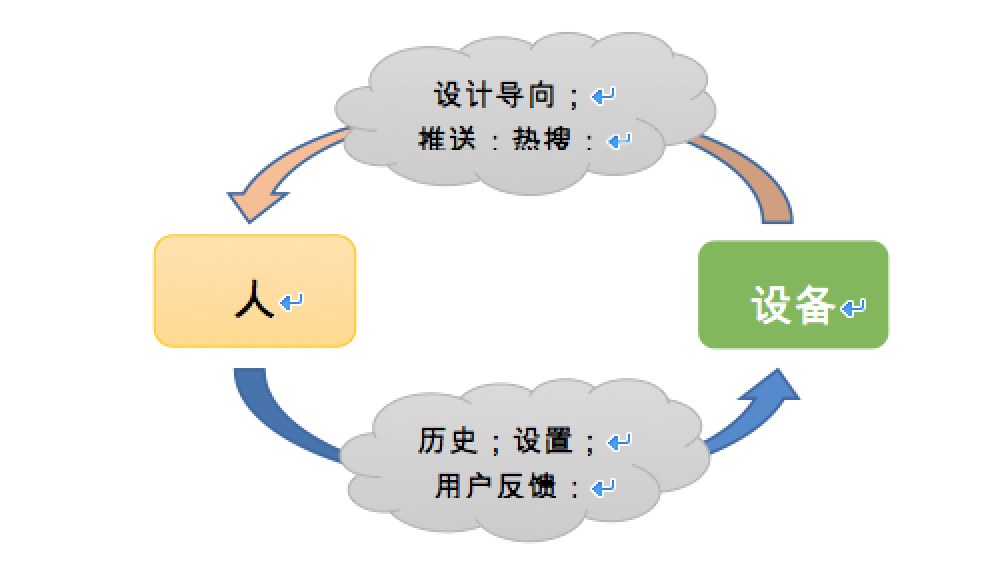
\includegraphics[scale=0.6]{人机交互}

如上图所示,软硬件设计本身就具有明显的导向性,例如抖音等小视频软件的诱导性,包括吸引用户发布视频和游客“沉浸”于浏览视频,微博等公众社交媒体“热搜”等设置有明显的舆论导向甚至价值导向作用;而用户的个人设置,浏览记录等信息使得媒体“更好地”针对性推送内容,使用户与设备的联系进一步加强,大数据背景下的用户反馈又是促使媒体优化设计的重要影响因素,使得“人机交互”成为一个持续的双向强化过程,并在这个过程中打造出一个针对用户个体的适宜、偏好和易沉浸的“强交互环境”。
\section{特征}

现象:设备使用频率和时长的增加
	在“人机强交互环境”中,人们对设备的使用频率在增加(时不时看手机),使用的持续时间变长(一看就是好几十分钟甚至几个小时),使用时的“浸入程度”也在加深(走路都要看,掉下水道里去!)。
		这中现象对人们的生活带来……的直接影响,也在悄然改变我们的思维和认知习惯……balabala……

\section{影响}
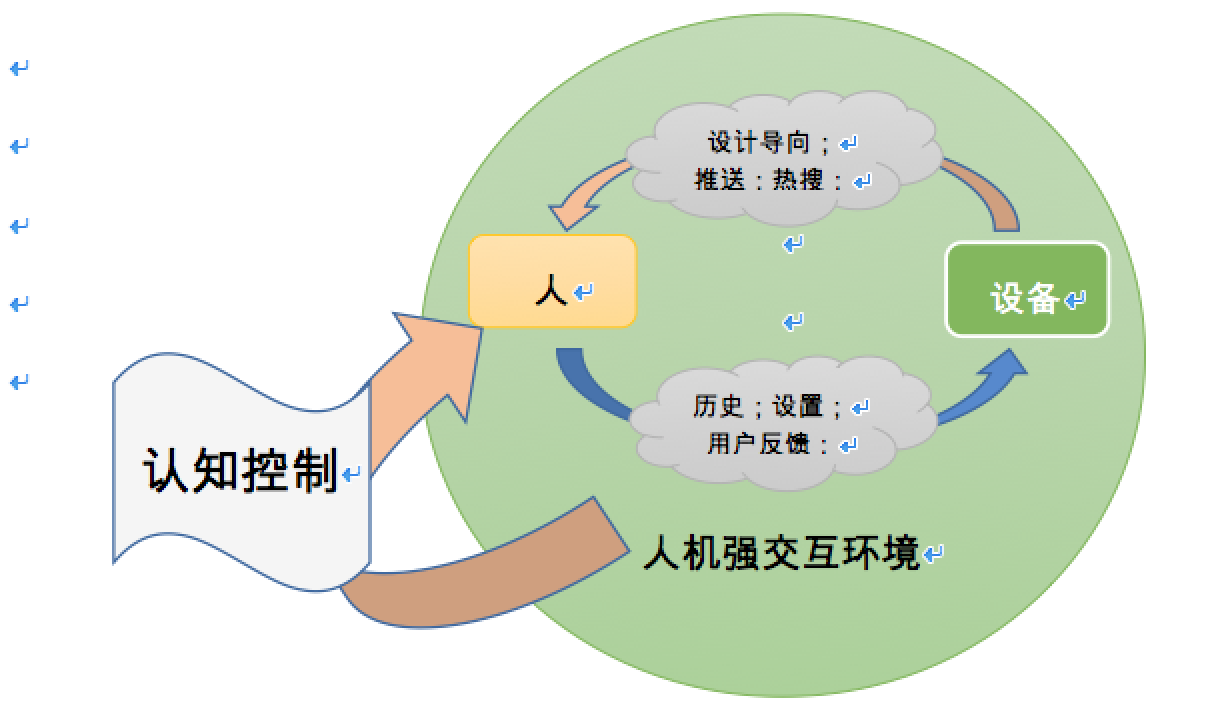
\includegraphics[scale=0.6]{人机强交互-认知控制}

当我们每天翻看手机上的社交平台,阅读那些看似有趣和有深度的文章时,我们正在渐渐丧失深度阅读和深度思考的能力。

互联网鼓励我们蜻蜓点水般地从多种信息来源中广泛采集碎片化的信息,其伦理规范就是工业主义,这是一套速度至上、效率至上的伦理,也是一套产量最优化、消费最优化的伦理。互联网正在按照自己的面目改造我们,我们变得对浏览和略读越来越得心应手,但是我们正在丧失的却是专注能力、沉思能力和反省能力。
